\section{Formative Study}
\label{sec:formative}

Before design was committed, a questionnaire and interviews tested whether the problem is real, whether the bounded design is a trust advantage, and which capabilities to build first.

\subsection{Method}
The questionnaire had 17 items in four areas: the respondent's context, the problem, design and trust, and feature demand, with Likert items on a 1 to 5 scale and a forced top-three selection from nine candidate features. It ran from 22 to 27 August 2026 through \InstitutionName{} student and practitioner networks and drew 374 valid responses. Thirteen in-person interviews were coded on five axes: the last time the participant lost their place, the workaround they already use, their reaction to the concept, what a trust-breaking mistake would do, and whether they would keep using the tool. The sample is 81 percent students and 13 percent developers, which matches the intended early-adopter profile but limits generalisation; 82 percent do multi-file work daily or a few times a week, and 77 percent had used an AI assistant. The system was described, not demonstrated, so predicted use and churn are stated intentions.
% TODO (team): add the consent and ethics statement your institution requires for this questionnaire and the interviews.

\subsection{Findings}
The problem is real. 44 percent of respondents often or always struggle to remember what they were doing when they return after a break, and only 7 percent never do. 59 percent agree their files become disorganised faster than they can clean them (mean 3.6). 42 percent lose more than an hour a week to reorientation, tidying, repeated tasks and searching scattered notes, and 14 percent more than three hours; the mode is 30 to 60 minutes, steady friction rather than crisis. Asked why the work is not already automated, 36 percent cited distrust of unsupervised automation and 28 percent not knowing how, against 24 percent for setup cost; the tasks exist, and what is missing is an instrument the user is willing to point at them.

The bounded design is a trust advantage. 65 percent rated an assistant that only sees files they explicitly add as meaningfully more trustworthy than one with full access (mean 3.8; Figure~\ref{fig:wstrust}). Local-first was the most common deployment preference at 40 percent, against 22 percent for cloud and 38 percent wanting specifics first, and the preference was consistent across students and developers (41 and 36 percent).

\begin{figure}[t]
  \centering
  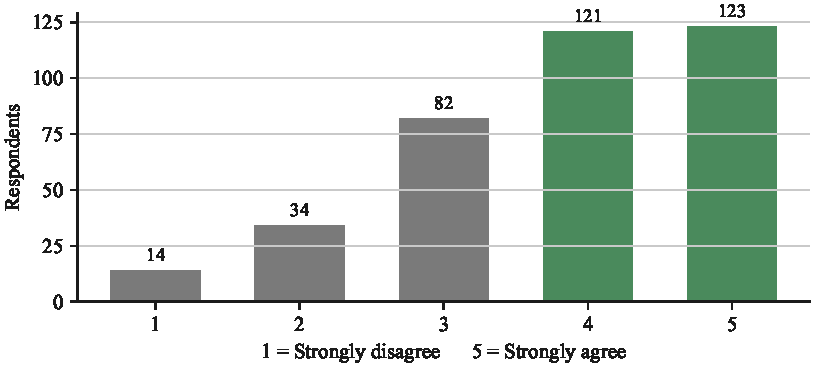
\includegraphics[width=\linewidth]{figures/fig_workspace_trust}
  \caption{Agreement that an assistant which only sees files explicitly added to a workspace is meaningfully more trustworthy than one with full access (1 = strongly disagree, 5 = strongly agree; 374 respondents).}
  \label{fig:wstrust}
\end{figure}

Users are divided on how much they wish to be asked. Offered a choice between an assistant that asks approval before every file change or outbound action and one that acts on reasonable requests with review and undo afterwards, respondents split 192 to 182. Role did not predict the preference; experience did, with regular AI-assistant users choosing approval-first less often than light users (44 against 59 percent). No single interaction model satisfies this population.

Users forgive a mistake they can reverse. 65 percent would keep using the assistant after one wrong or unwanted suggestion, and only 10 percent would abandon it. Predicted sustained use was moderate (47 percent likely, 22 percent unlikely, mean 3.3). The most predicted reasons for stopping were poor fit with existing habits (27 percent) and a mistake the user could not trust the tool to avoid again (24 percent), then redundancy with existing tools (20 percent) and privacy (17 percent); approval fatigue was the smallest named risk at 10 percent.

Demand is concentrated. Session resume (222 selections), multi-document synthesis (207) and folder tidy (200) led the forced top-three choice; code assistance followed (191); speech input and output was last by a wide margin (44). The most requested capability not on the roadmap was that the assistant learn the user's folder structure over time (18 mentions), followed by one-click universal undo (17). Seventeen free-text responses said the concept appeared already covered by existing coding assistants, and fifteen raised how much data is sent to a server. The interviews agreed: 10 of 13 reacted positively, 8 said a single mistake would not stop them, and effortless onboarding was the most named condition for continued use.

\subsection{Design implications}
Four decisions follow directly. Approval granularity is a user setting, not a product decision. Undo is a critical component shipped before any outward action. The bounded workspace and local-first default are kept and made visible in the product, which is also the answer to the redundancy objection. Learning the user's structure is specified as per-workspace memory that is visible and deletable, so personalisation stays inside the boundary. The build order was retained with synthesis brought forward, and speech kept last.
